\documentclass[10pt, a4paper]{article}

\usepackage[utf8]{inputenc}
\usepackage[english, spanish]{babel}
\usepackage[left=25mm, right=25mm, top=35mm, bottom=30mm, headheight=35mm]{geometry}
\usepackage{graphicx}
\usepackage{float}
\usepackage{xcolor}
\usepackage{fancyhdr}
\usepackage{hyperref}
\usepackage{setspace}
\usepackage{indentfirst}

% Syntax customization with minted package
\usepackage{minted}
\usemintedstyle{nord-darker}
\usemintedstyle[zsh]{gruvbox-light}
\setminted{
  breaklines,
  linenos,
  frame=lines,
  fontsize=\normalsize
}
\newcommand{\mpy}[1]{\mintinline[style=gruvbox-light]{python}{#1}}

% Define background color
\definecolor{background}{HTML}{2E3440}

% Variables
\newcommand{\university}{Universidad Nacional de San Agustín de Arequipa}
\newcommand{\faculty}{Facultad de Ingeniería de Producción y Servicios}
\newcommand{\program}{Escuela Profesional de Ingeniería de Sistemas}
\newcommand{\semester}{2024 - A}
\newcommand{\course}{img/web_programming.png}
\newcommand{\topic}{img/django_templates.png}
\newcommand{\professor}{Carlo Jose Luis Corrales Delgado}
\newcommand{\student}{Jorge Luis Mamani Huarsaya}
\newcommand{\email}{https://mail.google.com/mail/u/0/?fs=1&tf=cm&source=mailto&to=jmamanihuars@unsa.edu.pe}
\newcommand{\github}{https://github.com/jorghee/django-projects}
\newcommand{\mydate}{5 de junio, 2024}

% Just parts and chapters numbered
\setcounter{secnumdepth}{0}

% Head and foot customization
\pagestyle{fancy}
\lhead{\raisebox{-0.2\height}{
\includegraphics[width=4cm]{img/logo_unsa.png}}}
\chead{\fontsize{8}{8}\selectfont \university \\ \faculty \\ \textbf{\program}}
\rhead{\raisebox{-0.2\height}{
\includegraphics[width=3.5cm]{img/logo_episunsa.png}}}
\lfoot{Estudiante \student}
\cfoot{}
\rfoot{Pág. \thepage}

\begin{document}

\begin{titlepage}
	\centering
	\includegraphics[width=15cm]{\course} \par
  \vfill \vfill
	\includegraphics[width=15cm]{\topic}\par
  \vfill \vfill
  {\textbf{Profesor(a):} \par}
	\professor \vfill
  {\textbf{Estudiante:} \par}
	\student \vfill
  {\textbf{Email:} \par}
  \href{\email}{jmamanihuars@unsa.edu.pe} \vfill
  {\textbf{Repositorio GitHub:} \par}
  \href{\github}{\github} \vfill
	{\large \mydate \par}
\end{titlepage}

\section{Idea fundamental sobre cómo se comporta Django}
\begin{figure}[H]
  \centering
  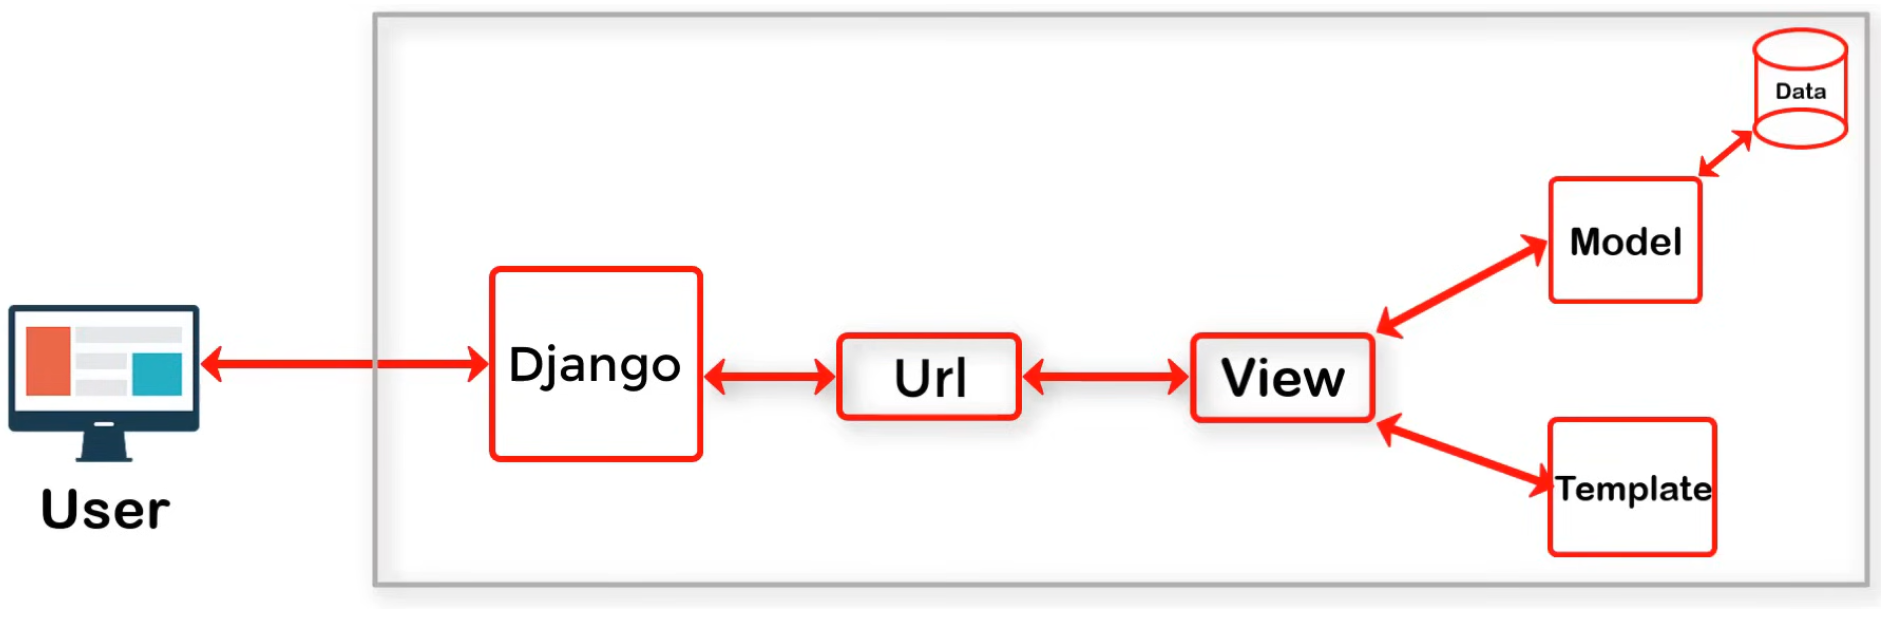
\includegraphics[width=0.8\textwidth]{img/model_view_template.png}
  \caption{Model View Template}
\end{figure}

\section{Agregando una plantilla HTML}
Lo primero que deseamos hacer es informarle a Django que deseamos servir archivos como lo son archivos HTML que en Django está bien definida y separada de la lógica del proyecto. Entonces comenzamos modificando el archivo \mpy{settings.py} del proyecto para definir el directorio en el cual se almacenarán los archivos HTML que representan la presentación del proyecto. Nos vamos directamente a la variable \mpy{TEMPLATES}.
\singlespacing
En la variable \mpy{TEMPLATES} agregamos un elemento al diccionario de clave \mpy{'DIRS'}

\begin{minted}[bgcolor=background]{python}
'DIRS': [os.path.join(BASE_DIR, 'templates')],
\end{minted}

La constante \mpy{BASE_DIR} es la dirección hasta el directorio raiz del proyecto.
\singlespacing
Una vez que tenemos configurada la dirección donde va a buscar Django las plantillas , podemos crear el directorio especificado y luego agregar un archivo \mpy{.html}. En este caso estamos utilzando una estructura ya definida y el archivo de inicio se denomina \mpy{index.html}. \textbf{Este archivo será el inicio de nuestra aplicación.}

\section{Agregando una vista para manejar el archivo index.html}
Siguiendo como es el funcionamiento de Django, ya hemos definido una Plantilla, por el momento no estamos definiendo trabajar con una base de datos, asi que nos toca definir \textbf{views}. Para ello nos posicionamos dentro de la Aplicación y modificamos el archivo \mpy{views.py}.

\begin{minted}[bgcolor=background]{python}
from django.shortcuts import render
from .models import Destination

def index(request):
  dests = Destination.objects.all()
  return render(request, "index.html", {'dests': dests})
\end{minted}

Como se observa, estamos definiendo una función que se encarga de obtener una lista de objetos que posteriormente se explicará a detalle, pero lo importante aqui es que esta retornando el archivo \mpy{index.html}. Además se está enviando la lista de objetos que, porsupuesto, serán usados en el archivo \mpy{index.html}.

\section{Mapeando las URLs en la Aplicación y en el Proyecto}
Ya abordamos el manejo de una solicitud especifica, sin embargo Django no sabe cómo recibir las solicitudes y direccionar existosamente. Por lo tanto, necesitamos crear el archivo \mpy{urls.py} dentro de la Aplicación y hacer las redirecciones correspondientes.

\begin{minted}[bgcolor=background]{python}
from django.urls import path
from . import views

urlpatterns = [
  path("", views.index, name="index")
]
\end{minted}

Como vemos, lo que se esta haciendo es establecer una ruta URL vacía (es decir, la página principal del proyecto) que será manejada por la vista index ubicada en el módulo views. El parámetro name="index" asigna un nombre a esta ruta, permitiendo que sea referenciada fácilmente en otras partes de la aplicación, como en plantillas HTML o redirecciones.
\singlespacing

\subsection{El archivo \mpy{urls.py} del proyecto}
Necesitamos que Django sepa cómo enrutar las solicitudes entrantes a las vistas correspondientes

\begin{minted}[bgcolor=background]{python}
from django.contrib import admin
from django.urls import path, include

urlpatterns = [
  path('', include('destinos_turisticos.urls')),
  path('admin/', admin.site.urls)
]
\end{minted}

Con esta configuración hacemos que todas las URLs definidas en la Aplicación, es decir en el archivo \mpy{urls.py} de dicha aplicación, sean accesibles desde la raiz de nuestro sitio web.
\singlespacing
Con estas modificaciones podemos lanzar nuestro servidor y nos daremos cuenta de que efectivamente el archivo \mpy{index.html} es encontrado, pero las hojas de estilos importadas y los scripts utilizados no son encontrados. 
\singlespacing
Entonces, ahora nos enfocamos en configurar un directorio especial que sirva \textbf{Archivos estáticos} como lo son los archivos .css, .js entre otros.

\section{Configuración de archivos estáticos}
Lo común en Django es crear un directorio nombrado como \mpy{static} donde se almacenarán todos los archivos estáticos, por lo tanto como hicimos anteriormente con el directorio \mpy{templates} necesitamos informarle a Django de esta configuración.

\begin{minted}[bgcolor=background]{python}
STATICFILES_DIRS = [
  os.path.join(BASE_DIR, 'static')
]
STATIC_ROOT = os.path.join(BASE_DIR, 'assets')
\end{minted}

Estas modificaciones la hacemos en el archivo \mpy{settings.py} del proyecto. Por el momento como solo tenemos una aplicación, estamos proporcionando este directorio \mpy{static} global para el proyecto, sin embargo una buena práctica es que cada Aplicación deba tener su propio directorio que almacene los archivos estáticos.
\singlespacing
El directorio especificado por \mpy{STATIC_ROOT} es donde Django recopila todos los archivos estáticos de la aplicación al ejecutar collectstatic. Esto centraliza los archivos para que puedan ser servidos eficientemente en producción por un servidor web. En este caso, se define como assets en el directorio base del proyecto.

\subsection{Modificando la dirección de los archivos importados en index.html}
Para brindar correctamente la dirección de los recursos que necesita el archivo \mpy{index.html} es necesario realizar las siguiente modificaciones:

\begin{minted}[bgcolor=background]{python}
<link rel="stylesheet" type="text/css" href="">
\end{minted}

El uso de \mpy{static} en el enlace es necesario para construir correctamente la URL de los archivos estáticos. Django reemplaza \mpy{{\% static \%}} con la URL base definida en \mpy{STATIC_URL}, asegurando que el navegador pueda encontrar y cargar el archivo CSS, independientemente del entorno (desarrollo o producción).

\section{Definiendo Modelos usando el sistema de gestión de base de datos PostgreSQL}
Hasta el momento no hemos utilizando en ningún momento Base de datos, sin embargo Django nos brinda una forma muy limpia de poder realizar operaciones en la base de datos sin la necesidad de usar el lenguaje \mpy{sql}.
\singlespacing
Recordemos el modelo de trabajo de Django, ahora vamos a definir el concepto de \mpy{Model}. Para ello, nos vamos al archivo \mpy{models.py} de la Aplicación, y aqui podemos definir una clase como un modelo en Django. Un modelo en este framework es una clase que representa una tabla en la base de datos. 

\begin{minted}[bgcolor=background]{python}
from django.db import models

class Destination(models.Model):
  name = models.CharField(max_length=100)
  img = models.ImageField(upload_to='pics')
  desc = models.TextField()
  price = models.IntegerField()
  offer = models.BooleanField(default=False)
\end{minted}

\begin{itemize}
  \item \textbf{name:} Un campo de texto (CharField) con un máximo de 100 caracteres.
  \item \textbf{img:} Un campo de imagen (ImageField) que almacena la ruta de la imagen en el directorio \mpy{pics}.
  \item \textbf{desc:} Un campo de texto largo (TextField) para descripciones.
  \item \textbf{price:} Un campo entero (IntegerField) para precios.
  \item \textbf{offer:} Un campo booleano (BooleanField) que indica si hay una oferta, con un valor predeterminado de \mpy{False}.
\end{itemize}

Lo interesante de este modelo es que todas las instancias de esta clase van a ser los destinos destinos turísticos de nuestro sitio web. Recordemos al momento de definir la función \mpy{index()} en el archivo \mpy{views.py} donde estuvimos obteniendo todos los objetos instanciados en la clase \mpy{Destination}, que básicamente estamos recuperando las filas de la base de datos.

\section{Usando los objetos enviados al navegador en el archivo index.html}
En la plantilla nosostros podemos iterar por la lista de objetos que se han enviando, este es una característica especifica de los sistemas de plantillas de Django, una funcionalidad valiosa.

\begin{minted}[bgcolor=background]{python}

<div class="destination item">
  <div class="destination_image">
    <img src="{{dest.img.url}}" alt="">
    
    <div class="spec_offer text-center"><a href="#">Oferta especial</a></div>
    
  </div>
  <div class="destination_content">
    <div class="destination_title"><a href="destinations.html">{{dest.name}}</a></div>
    <div class="destination_subtitle"><p>{{dest.desc}}</p></div>
    <div class="destination_price">Desde S/. {{dest.price}}</div>
  </div>
</div>

\end{minted}

Como vemos, estamos iterando sobre la lista de objetos, además estamos usando un condicional para agregar una etiqueta que informa si el tour esta en oferta o no. Recordemos que el campo \mpy{offer} está almacenda en la base de datos como un dato booleano.

\section{Creando un Administrador}
El Administrador debe tener la capacidad de poder modificar, insertar y eliminar destinos turísticos. Django proporciona una interfaz de administración incorporada que nos permite a nosotros los desarrolladores crear rápidamente una interfaz de administración básica para nuestras aplicaciones web sin necesidad de escribir código adicional.
\singlespacing
Lo único que vamos a hacer es registrar el Modelo \mpy{Destination} en la interfaz de administración de Django. 

\begin{minted}[bgcolor=background]{python}
from django.contrib import admin
from .models import Destination

admin.site.register(Destination)
\end{minted}

Este registro habilita la administración básica de los objetos \mpy{Destination}, como la creación, edición y eliminación de registros, a través de la interfaz de administración de Django, que está disponible en la ruta predeterminada \textbf{/admin} del sitio web.

\end{document}
